%Appendix_spot_size
In this section we will introduce the process of calculating beam spot size from data in CST MWS. As definition of spot size, the target is the distance from beam center to the point where the power density is $1/e^{2}$ of the peak value.  Fig. \ref{Afig:beam_cuboid} is the calculation cuboid in the CST MWS. The Gaussian beam propagates along the z-axis in the simulation of this work. So the spot diameter is the function of z coordinate $d=f(z)$. In order to calculate the spot diameter we cut a working plane at each z-coordinate. Like the step in Appendix \ref{app:powwer_distribution}, we assume a working plane through the point $z_{0}$. In this work the simulation of beam propagation is symmetric on both x-axis and y-axis. Thus only quarter of the beam cross-section is the working plane like Fig. \ref{Afig:beam_crosssection} in CST MWS. Supposing the point $n_{0}$ is the beam center of this plane the peak value of the power flow density is $|S(n_{0})|$. The next step is to find the point $n_{1}$ where $|S(n_{1})|=1/e^{2}|S(n_{0})|$. $n_{1}$ is also among the range $[n_{0}, n_{0}+n_{x}n_{y}]$. Point $n_{1}$ leads to its coordinate ($x_{1},y_{1}$). Then the beam spot radium of this plane is given by \ref{eq:spot_radium}. The spot size is twice of this radium. We can draw the spot size curve by joining values of the spot size in each cross-section.
\begin{figure}[!ht]
\centering
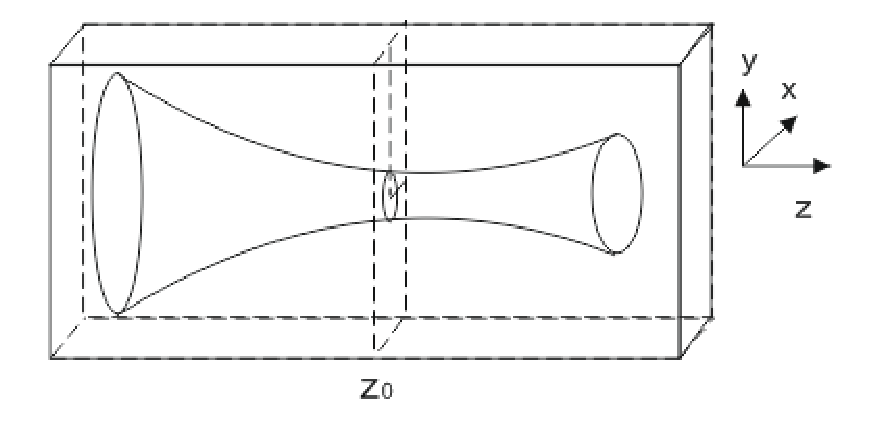
\includegraphics[width=0.5\textwidth]{bilder/beam_cuboid}
\caption{Beam propagation in simulation cuboid.}
\label{Afig:beam_cuboid}
\end{figure}
\begin{figure}[!ht]
\centering
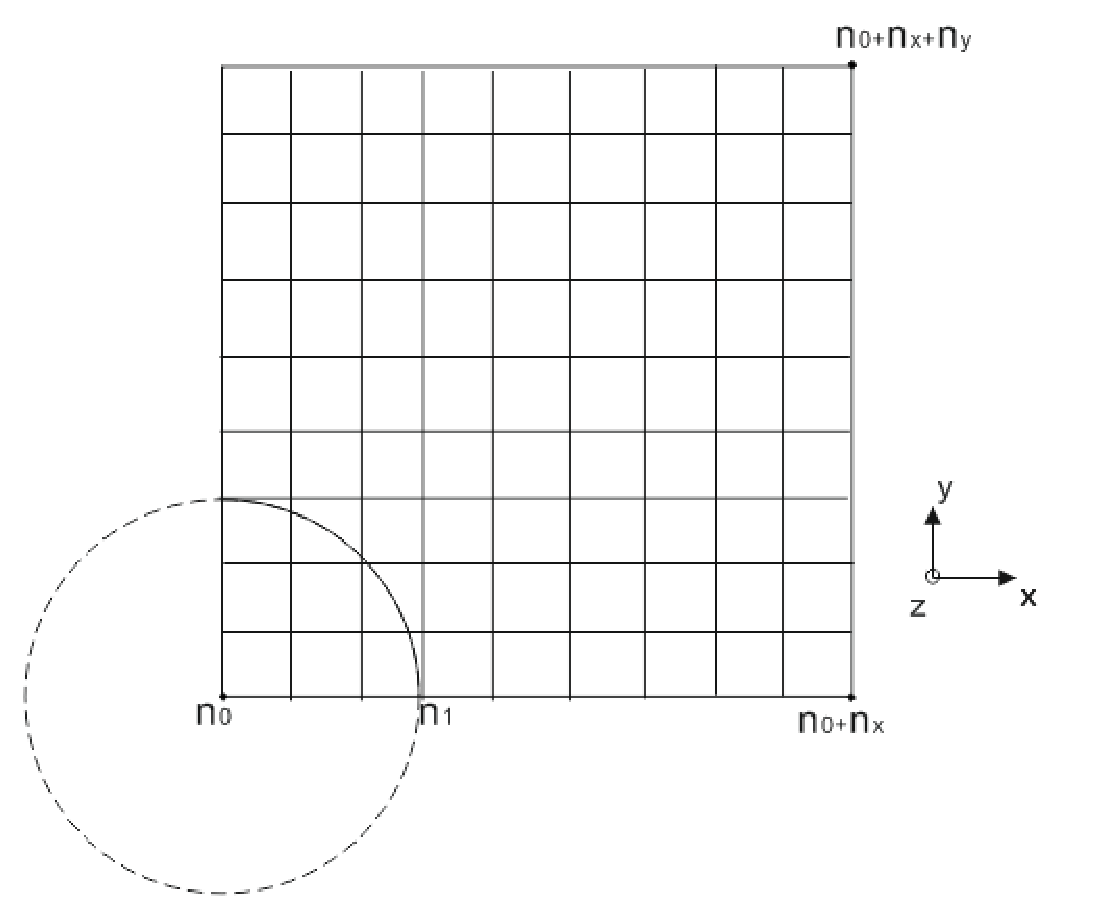
\includegraphics[width=0.5\textwidth]{bilder/beam_crosssection}
\caption{Beam cross-section at through point $n_{0}$.}
\label{Afig:beam_crosssection}
\end{figure}
\begin{equation}
R=\sqrt(x_{1}^{2}+y_{1}^{2})
\label{eq:spot_radium}
\end{equation} 
